\documentclass[xcolor={dvipsnames}]{beamer}
\mode<presentation>
{
  \usetheme{Antibes}      % or try Darmstadt, Madrid, Warsaw, ...
  \usecolortheme{dolphin} % or try albatross, beaver, crane, ...
  \usefonttheme{professionalfonts}  % or try serif, structurebold, ...
  \setbeamertemplate{navigation symbols}{}
  \setbeamertemplate{caption}[numbered]
} 
\usepackage[utf8]{inputenc}
\usepackage[english]{babel}
\usepackage{multirow}
\usepackage{subfigure}
\usepackage{color}
\graphicspath{{/D:/fh/JI/latex/VE230 slides}}
\usepackage{amsmath}
\title[VE230 RC slides week 1]{VE230 RC slides Week 2}
\author{han.fang }
\date{\today}

\begin{document}
\begin{frame}
\titlepage
\end{frame}


\begin{frame}{Course Overview}
\begin{block}{Course overview}
\begin{itemize}
	\item Integral
	\item Fields
	\item Assignment 2
\end{itemize}
\end{block}
\end{frame}
\begin{frame}{Integral}
\begin{block}{Line integrals}
When integrated along a certain differential length, use equations we introduced last class to convert differential length to integrable quantities with regard to different coordinates. For example, in Cartesian coordinates, when integrating on $d\vec{l}$, you should convert $d\vec{l}$ into the form
$$d\vec{l} = \vec{a_x}dx + \vec{a_y}dy + \vec{a_z}dz.$$
\end{block}
\end{frame}
\begin{frame}{Integral}
\begin{block}{A small example}
Suppose $\vec{F}=\vec{a_x}xy - \vec{a_y}2x$, calculate its integral along $y=x^2$ in the range [0,1].
\end{block}
\pause 
\begin{block}{Answer}
\[
\begin{aligned}
W&=\int \vec{F}\cdot d\vec{l}\\
&=\int (\vec{a_x}xy - \vec{a_y}2x)\cdot (\vec{a_x}dx + \vec{a_y}dy)\\
&=\int xydx-2xdy\\
&=\int_0^1 (x*x^2dx-2x*2xdx)=-\frac{13}{12}\\
\end{aligned}
\]
\end{block}
\end{frame}
\begin{frame}{Integral}
Flux: the integrals of the vector field rush out the surface.
\begin{figure}[H]
	\centering
	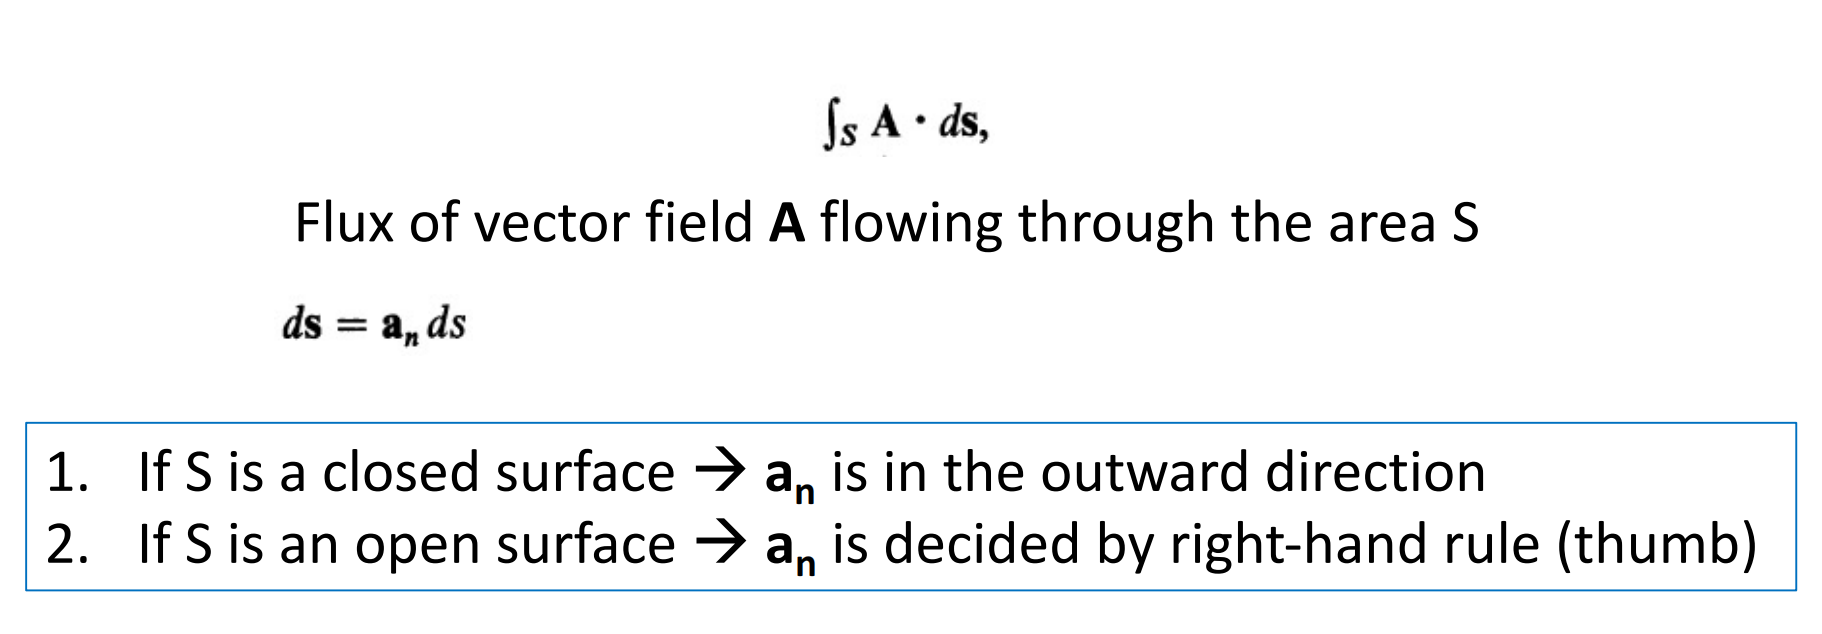
\includegraphics[width=0.7\linewidth]{2_1.png}
\end{figure}
\end{frame}
\begin{frame}{Scalar field and vector field}

\begin{block}{Scalar field}
The intensity of the field is a scalar value, for example, gravitation potential field.
\end{block}
\pause
\begin{block}{Vector field}
The intensity of the field is a vector value, for example, gravitational field.
\end{block}
\pause
\begin{block}{Connection}
The vector field can be the gradient of a scalar field.
\end{block}
\end{frame}
\begin{frame}{Gradient of a scalar field}

\begin{itemize}
    \item $$\nabla V = \vec{a_n} \frac{dV}{dn}$$
    \item $\nabla V$ at certain point is a vector.
    \item $$dV = (\nabla V)\cdot d\vec{l}$$: the space rate of increase of $V$ in the $\vec{a_l}$ direction is equal to the projection (the component) of the gradient of $V$ in that direction. 
    \item $$
        \nabla V = \vec{a_{u1}} \frac{\partial V}{h_1\partial u_1} + \vec{a_{u2}}\frac{\partial V}{h_2\partial u_2} + \vec{a_{u3}} \frac{\partial V}{h_3\partial u_3}
    $$, when $V$ is taken off:
    $$
    \nabla \equiv  \vec{a_{u1}} \frac{\partial }{h_1\partial u_1} + \vec{a_{u2}}\frac{\partial }{h_2\partial u_2} + \vec{a_{u3}} \frac{\partial }{h_3\partial u_3}
    $$
\end{itemize}
\end{frame}
\begin{frame}{Divergence of a vector field}
\begin{itemize}
    \item divergence of a vector field $\vec{A}$ at a point $div\vec{A}$ as the net outward flux of $\vec{A}$ per unit volume as the volume about the point tends to zero: 
    \begin{equation}\label{Eq: definition-divergence-of-vector-field}
        div\vec{A} = \lim_{\Delta v\to 0}\frac{\oint\limits_{S}\vec{A}\,\mathrm{d}s}{\Delta v} 
    \end{equation}
 
    \item source: net positive divergence; sink: net negative divergence. zero divergence: no source/sink.
    \item $div\vec{A}$ at certain point is a scalar.
\end{itemize}

\end{frame}
\begin{frame}{Divergence of a vector field}
\begin{itemize}
    \item For Cartesian coordinate, 
    $$div\vec{A} = \frac{\partial A_x}{\partial x} + \frac{\partial A_y}{\partial y} + \frac{\partial A_z}{\partial z}$$
    \item $$\nabla \cdot \vec{A} \equiv div \vec{A}$$
    \item $$\nabla \cdot \vec{A} = \frac{1}{h_1h_2h_3}[\frac{\partial}{\partial u_1}(h_2h_3A_1)+\frac{\partial}{\partial u_2}(h_1h_3A_2)+\frac{\partial}{\partial u_3}(h_1h_2A_3)]$$
\end{itemize}
\end{frame}
\begin{frame}{Divergence Theorem}
\begin{itemize}
    \item $$\int_V\nabla\cdot \vec{A}dv = \oint_S\vec{A}\cdot d\vec{s}$$, the volume integral of the divergence of a vector field equals the total outward flux of the vector through the surface that bounds the volume.
    \item A most famous theorem in the physics - Gauss's law can be deduced by divergence theorem very easily. Thus, the divergence theorem will be quite fundamental in this course. Make sure you understand it.
\end{itemize}
\end{frame}
\begin{frame}{Curl of a vector field}
\begin{itemize}
    \item $$curl \vec{A}\equiv\nabla\times\vec{A}=\lim_{\Delta s\to 0}\frac{1}{\Delta s}[\vec{a_n}\oint_{C}\vec{A}\cdot d\vec{l}]_{max}$$: the curl of a vector field $\vec{A}$, denoted by $curl\vec{A}$ or $\nabla\times\vec{A}$, is a vector whose magnitude is the maximum net circulation of $\vec{A}$ per unit area as the area tends to zero and whose direction is the normal direction of the area when the area is oriented to make the net circulation maximum. (Right hand rule defines the positive normal to an area).
    \item $\nabla\times\vec{A}$ in a general coordinate:
    $$
    \nabla\times\vec{A}=\frac{1}{h_1h_2h_3}\begin{vmatrix}
        \vec{a_{u1}}h_1 & \vec{a_{u2}}h_2 &\vec{a_{u3}}h_3\\
        \frac{\partial}{\partial u_1} & \frac{\partial}{\partial u_2} &\frac{\partial}{\partial u_3}\\
        h_1A_1 & h_2A_2 & h_3A_3
    \end{vmatrix}
    $$
    \item curl-free vector field ($\nabla\times\vec{A}=0$): \textbf{irrotational} or \textbf{conservative field}, like the gravitation potential field.
\end{itemize}
\end{frame}
\begin{frame}{Stokes's Theorem}
\begin{itemize}
    \item $$\int_S(\nabla\times\vec{A})d\vec{s}=\oint_C\vec{A}\cdot d\vec{l}$$: the surface integral of the curl of a vector field over an open surface is equal to the closed line integral of the vector along the contour bounding the surface.
\end{itemize}
\end{frame}
\begin{frame}{Other Identities}
\begin{itemize}
    \item[I]
    \begin{itemize}
        \item $$\nabla\times(\nabla V) \equiv 0$$: the curl of the gradient of any scalar field is identically zero.
        \item Another interpretation: If a vector field is curl-free, it can be expressed as the gradient of a scalar field.
        \item Since a curl-free vector field is irrotational or conservative, an irrotational/conservative vector field can always be expressed as the gradient of a scalar field.
    \end{itemize} 
    \item[II]\begin{itemize}
        \item $$\nabla\cdot(\nabla\times\vec{A})\equiv0$$: the divergence of the curl of any vector field is identically zero.
        \item Another interpretation: if a vector field is divergenceless, it can be expressed as the curl of another vector field.
        \item Divergenceless field is called solenoidal field, which will be further discussed in later classes.
    \end{itemize}
\end{itemize}
\end{frame}
\begin{frame}{Other Identities}
\begin{block}{Laplacian in Cartesian Coordinates}
$$\nabla^2 V = \frac{\partial^2 }{\partial x^2}+\frac{\partial^2 }{\partial y^2}+\frac{\partial^2 }{\partial z^2}$$
\end{block}
\pause
\begin{block}{Helmholtz's Theorem}
Any vector in 3D can be decomposable into a sum of the following vector fields. A vector field (vector point function) is determined to within an additive constant if both its divergence and its curl are specified everywhere.
$$F=-\nabla V+\nabla\times A.$$
\end{block}
\end{frame}
\begin{frame}{Other useful vector properties}
\begin{figure}[H]
	\centering
	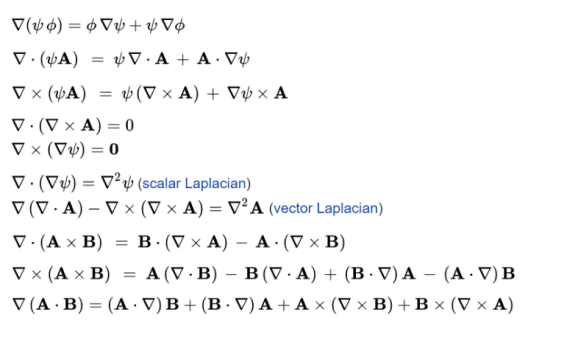
\includegraphics[width=0.9\linewidth]{2_3.png}
\end{figure}
\end{frame}
\begin{frame}{About the Assignments}
	I hope you don't just copy the answer I showed, but instead tried to understand the problem. In order to make sure the quality of other 2 RCs, the slides I submit on canvas will be without the answer. But you don't need to take the screen shot, since the answer will be released after the deadline. Also, for those students who just want to copy the answer, it is a waste of time, since the assignments will not be counted into the final.
\end{frame}
\begin{frame}{Assignments}
\begin{block}{\textbf{P.3-8}}
A line Charge of uniform density $\rho_l$ in free space forms a semicircle of radius b. Determine the magnitude and direction of the electric field intensity at the center of the semicircle.
\end{block}
\pause
\begin{figure}[H]
	\centering
	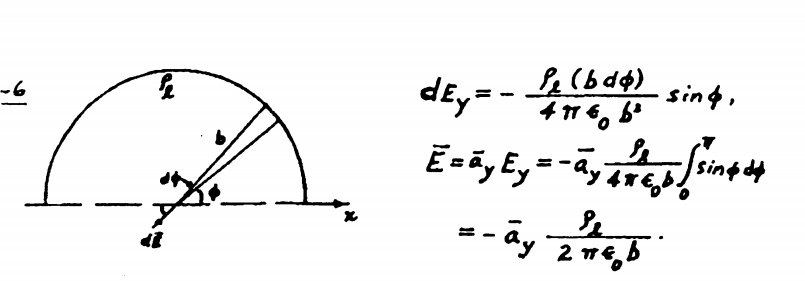
\includegraphics[width=0.7\linewidth]{2_4.png}
\end{figure}
\end{frame}
\begin{frame}{Assignments}
\begin{block}{\textbf{P.3-9}}
Three uniform line charges-- $\rho_{l_1},\rho_{l_2}$, and $\rho_{l_3}$, each of length L--form an equilateral triangle. Assuming that $\rho_{l_1}=2\rho_{l_2}=2\rho_{l_3}$, determine the electric field intensity at the center of the triangle.
\end{block}
\pause
\begin{figure}[H]
	\centering
	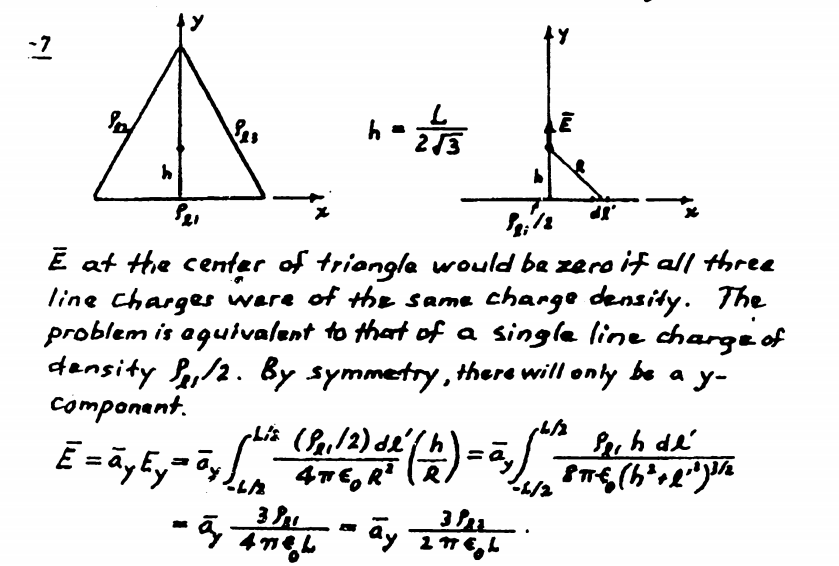
\includegraphics[width=0.7\linewidth]{2_5.png}
\end{figure}
\end{frame}
\begin{frame}{Assignments}
\begin{block}{\textbf{P.3-12}}
Two infinitely long coaxial cylindrical surfaces, $r=a$ and $r=b (b>a)$, carry surface charge densities $\rho_{sa}$ and $\rho_{sb}$, respectively.\\
\textbf{a)} Determine \textbf{E} everywhere.\\
\textbf{b)} What must be the relation between a and b in order that \textbf{E} vanishes for $r>b$?
\end{block}
\pause
\begin{figure}[H]
	\centering
	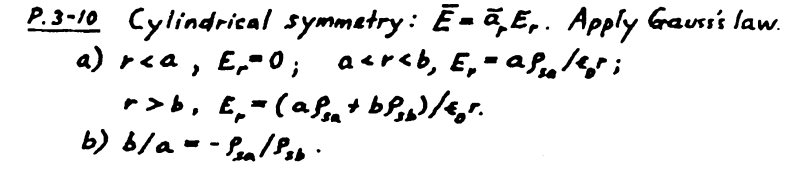
\includegraphics[width=0.7\linewidth]{2_6.png}
\end{figure}
\end{frame}
\begin{frame}{Assignments}
\begin{block}{\textbf{P.3-13}}
Determine the work done in carrying $a - 2(\mu C)$ charge from $P_1$(2,1,-1) to $P_2(8,2,-1)$ in the field $\boldsymbol{E}=\boldsymbol{a_x}y+\boldsymbol{a_y}x$.\\
\textbf{a)} along the parabola $x=2y^2$\\
\textbf{b)} along the straight line joining $P_1$ and $P_2$.\\
\end{block}
\pause
\begin{figure}[H]
	\centering
	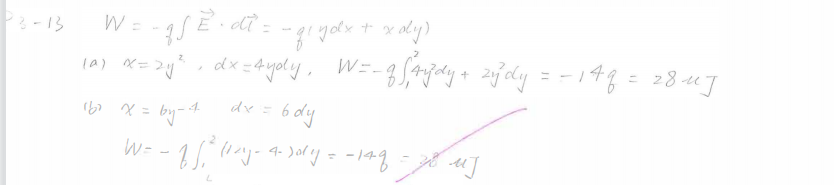
\includegraphics[width=0.9\linewidth]{2_7.png}
\end{figure}
\end{frame}
\begin{frame}{Assignments}
\begin{block}{\textbf{P.3-16}}
A finite line charge of length $L$ carrying uniform line charge density $\rho_l$ is coincident with the x-axis.\\
\textbf{a)} Determine V in the plane bisecting the line charge.\\
\textbf{b)} Determine \textbf{E} on the bisecting plane from $\rho_l$ directly by applying Coulomb's law.\\
\textbf{c)} Check the answer in part(b) with $-\nabla V$.\\
\end{block}
\pause
\begin{figure}[H]
	\centering
	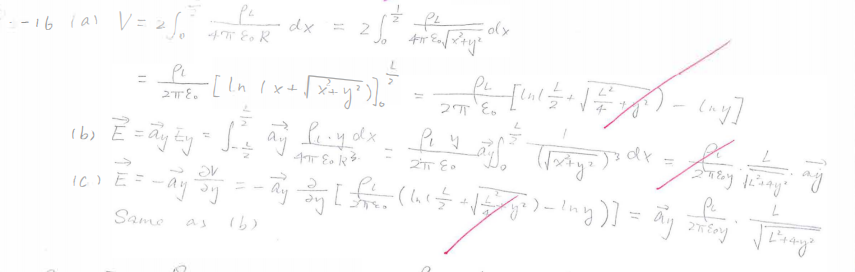
\includegraphics[width=0.9\linewidth]{2_8.png}
\end{figure}
\end{frame}
\begin{frame}{Assignments}
\begin{block}{\textbf{P.3-19}}
A charge $Q$ is distributed uniformly over the wall of a circular tube of radius $b$ and height $h$. Determine $V$ and \textbf{E} on its axis.\\
\textbf{a)} at a point outside the tube, then\\
\textbf{b)} at a point inside the tube.\\
\end{block}
\pause
\begin{figure}[H]
	\centering
	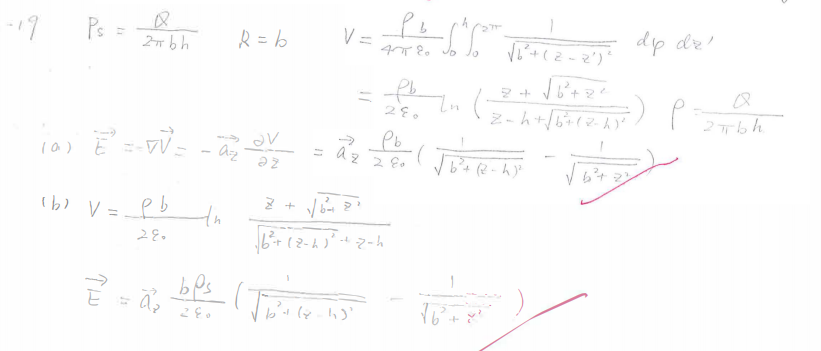
\includegraphics[width=0.9\linewidth]{2_9.png}
\end{figure}
\end{frame}
\end{document}